\documentclass[12pt,a4paper]{article}
\usepackage[utf8]{inputenc}
\usepackage[french]{babel}
\usepackage[T1]{fontenc}
\usepackage{amsmath}
\usepackage{amsfonts}
\usepackage{amssymb}
\usepackage{graphicx}
\usepackage[left=2cm,right=2cm,top=2cm,bottom=2cm]{geometry}
\author{KONDI Abdoul malik \\ NGANDEU NDJEUKAM Alhasan}
\title{Rapport du stage de fin L2}
\begin{document}
\maketitle
\tableofcontents
\newpage

\section{Introduction}
Dans le cadre d'améliorer nos compétence technique mais surtout professionnel, il nous a expressément été demander de faire un stage de mise en pratique d'une durée de six semaine dans une organisation de notre choix. C'est dans cette optique que nous nous somme présenté pour être stagiaire à la \textbf{médiathèque} afin de répondre à leurs besoins.
Le but de notre stage était de réaliser une application de gestion d'ouvrages à la  bibliothèque de la médiathèque.
Ce rapport détail le déroulement de notre stage notamment comment nous nous somme pris pour analyser le besoin exprimé par l'organisation, comment nous avons réaliser le modèle répondant au besoin décrit par cette dernière et enfin les difficultés que nous avons rencontré ainsi que les améliorations futur. Ainsi nous allons parler de l'organisme qui nous à accueillie : la médiathèque.

\section{Organisme d'accueil}
%présenter l'organisation d'accueil
\textbf{Urbis Foundation} est une organisation non gouvernemental crée à Munich en Allemagne en 2002 avec pour objectif la protection internationale du climat et de l’environnement qui s'est installé dans la région central et est situé a quelques mètre de la route national N°1 en face de la mairie de sokodé. Cet organisme installa à Sokodé, une médiathèque associé à une bibliothèque contenant les livres scolaires accessibles en présentiel par des élèves, des étudiants et des professionnels.En effet cet organisme dispose d'une médiathèque avec des livres, des journaux, des supports audio et vidéo d'autant plus que chaque ouvrage est fournis en plusieurs exemplaires. Ainsi pour assurer le bon fonctionnement et atteindre ces objectifs Urbis Foundation a mis en place une structure bien défini ayant en tête un \textbf{Conseil de Fondation UF Allemagne}, suivis d'un \textbf{Conseil d’Administration UF Togo} puis d'un \textbf{Direction Générale}. Deux catégorie se place sous le Direction Générale il s'agit du \textbf{Secrétariat Général} et de la \textbf{Comptabilité}. Sous ces deux catégories figurent des secteurs à savoir le \textbf{Secteur énergie solaire}, le \textbf{Secteur Santé}, le \textbf{Secteur environnement et agriculture(ferme école CPIA)}, le \textbf{Secteur éducation et formation professionnelle (Médiathèque)}, puis le \textbf{Secteur action sociale et humanitaire}. Dans le secteur de L’Énergie solaire nous distinguons deux volets à savoir le \textbf{Volet formation} ainsi que \textbf{Volet installation}. Dans le secteur de l'environnement et de l'agriculture nous distinguons 4 volets à savoir le \textbf{Volet Elevage}, le \textbf{Volet Agriculture}, le \textbf{Volet Arboriculture}, et le \textbf{Volet Maraichage}. Dans le Secteur éducation et formation professionnelle (Médiathèque), nous distinguons 3 Volets à savoir le \textbf{Volet Formation}, le \textbf{Volet Secrétariat} et le \textbf{Volet Bibliothèque}. Dans le secteur Secteur action sociale et humanitaire nous distinguons 2 Volets à savoir le \textbf{Volet Micro-credit} et le \textbf{Volet Parrainage}. Puis comme sous volet du volet Secrétariat nous avons les \textbf{Gardiens} et les \textbf{Femmes de ménages}. Lors de notre Stage nous avons demeuré dans les locaux d'Urbis afin de mieux appréhender leur besoin et d'être en parfaite collaboration, à cet effet dans les locaux de Urbis nous avons été logé dans le \textbf{Volet Bibliothèque} du point de vu du besoin exprimé par Urbis car dans ce volet nous devons nous charger d'apporter quelques modifications à leur bibliothèque en la modernisant et en mettant en place en plus de celle qui existe une bibliothèque accessible en ligne.\\

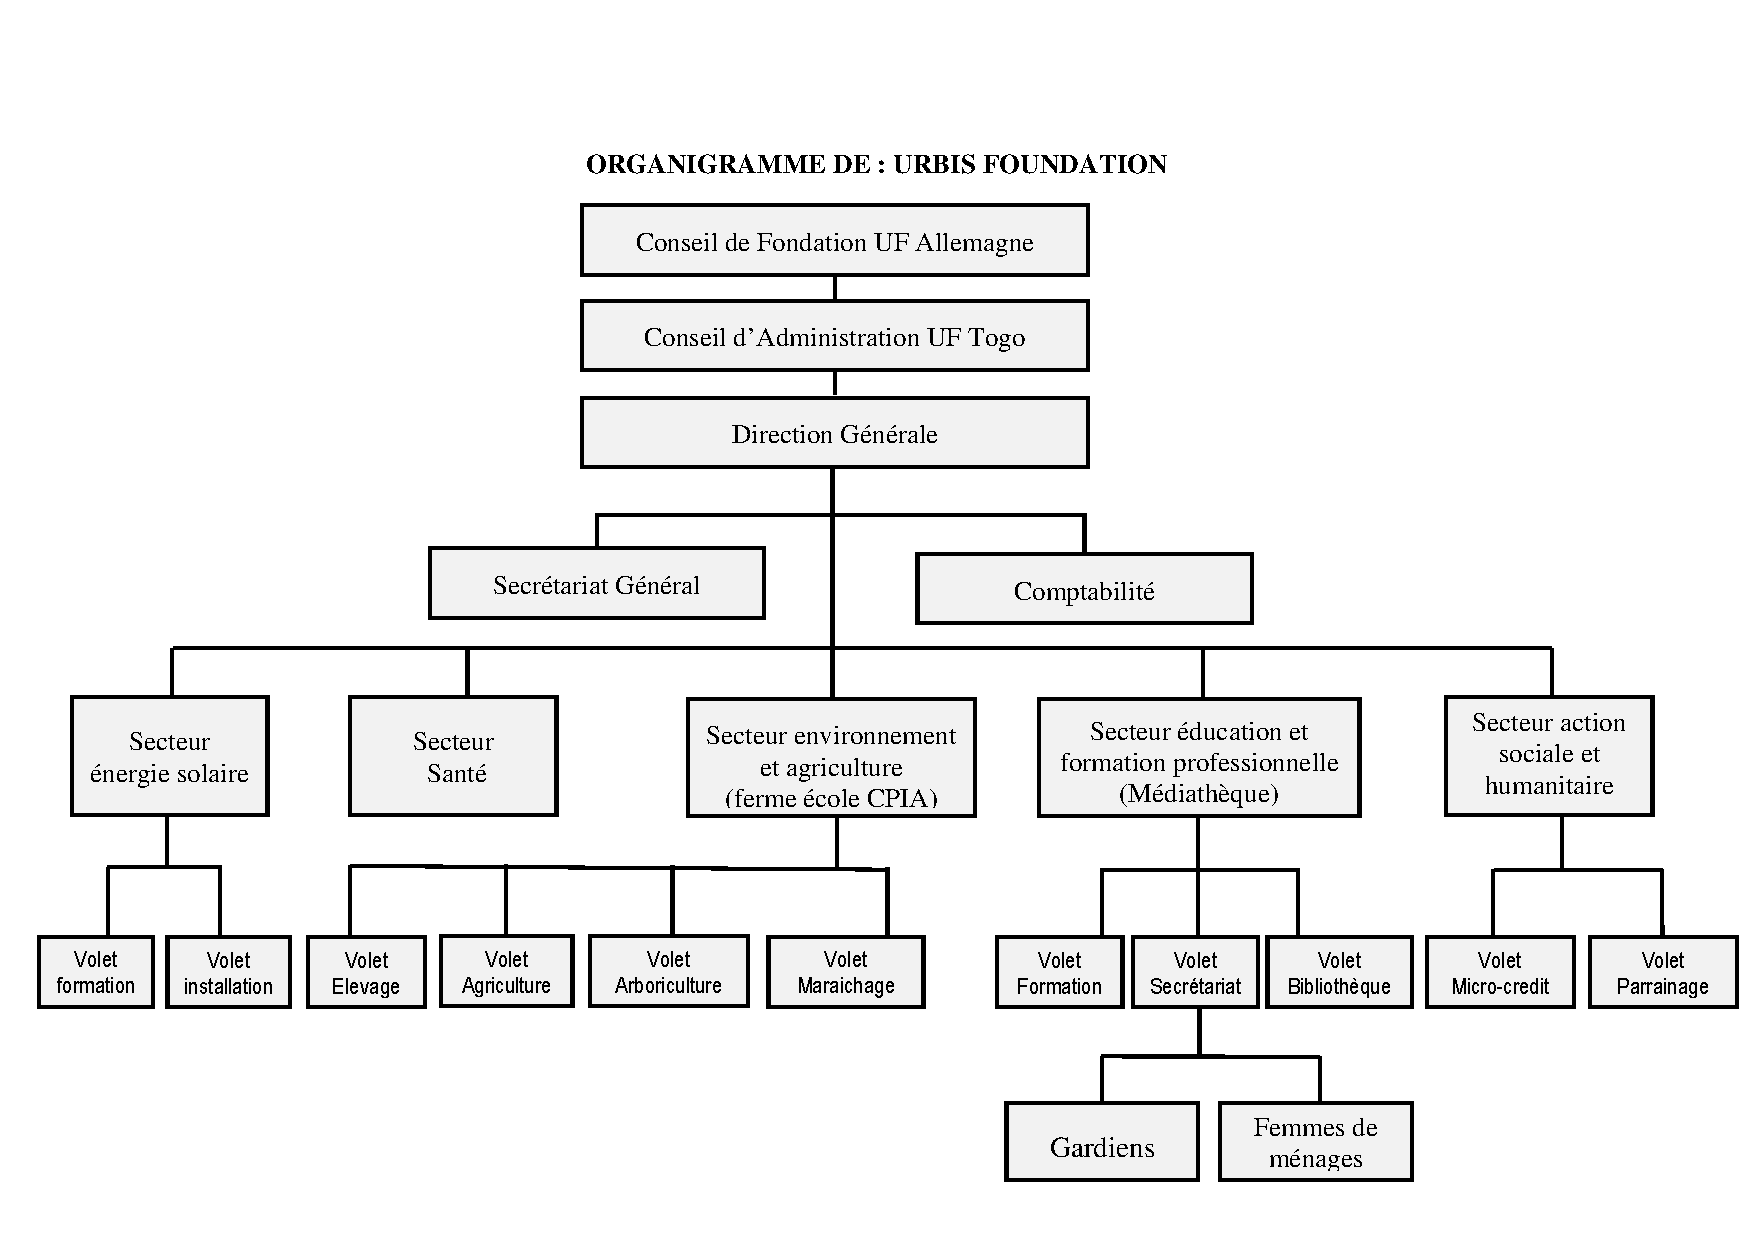
\includegraphics[width=16cm,height=15cm]{./images/ORGANIGRAMME.pdf} 
%organimagramme complet identifiant le service dans le quelle le stagier à travailé.
\newpage
\section{Analyse et modélisation du problème}
L'objectif de notre stage à la médiathèque était de mettre en place une bibliothèque accessible en ligne. Pour pouvoir y parvenir, nous avons du principalement dans les deux premières semaines du stage travailler avec le personnel de la bibliothèque pour pouvoir construire un modèle solide. A l'issue 
de ce travaille nous avons réaliser un diagramme de cas d'utilisation et un 
diagramme de classe. Ces diagrammes (surtout le diagramme de classe) ont évolué
au cours du stage. Nous allons donc parler plus en détails de chacune d'entre d'elle.

\subsection{Diagramme de cas d'utilisation}
Le diagramme de cas d'utilisation comme vous le savez déjà décrit toute les actions
possible pour chaque personne (acteur) ayant accès à l'application (au système). Dans 
notre cas pour réaliser ce diagramme nous nous sommes basé essentiellement sur les besoins décrit dans le cahier des charges à savoir : 
\begin{itemize} 
\item[•] Enregistrer de nouvels abonnés et de les classer dans une catégorie (élève, étudiant, professionnel...) ;
\item[•] Permettre au gérant de la médiathèque de gérer les prêts des ouvrages physiques pour les abonnés ;
\item[•] Possibilité pour les utilisateurs de consulter en ligne plus de 2000 livres ;
\item[•] Pouvoir déclencher la recherche d’un livre à l’aide du titre, des mots-clés, de l’auteur, de l’année
de parution du livre, de son type, du domaine auquel il s’applique etc... ;
\item[•] Donner la possibilité aux utilisateurs de la bibliothèque numérique de télécharger des livres au
format PDF ;
\item[•] Pouvoir ajouter de nouveaux livres en saisissant l’ISBN ;
\end{itemize}
Plus tard pendant la phase d'analyse ont été ajouté les besoins suivant.\\
\begin{itemize}
\item[•] La gestion des réservations en ligne de livre physique.
\item[•] L'implémentation d'un serveur de messagerie pour alerter les abonnés afin
que ces dernier puissent ramener les ouvrages emprunté à temps.
\end{itemize}
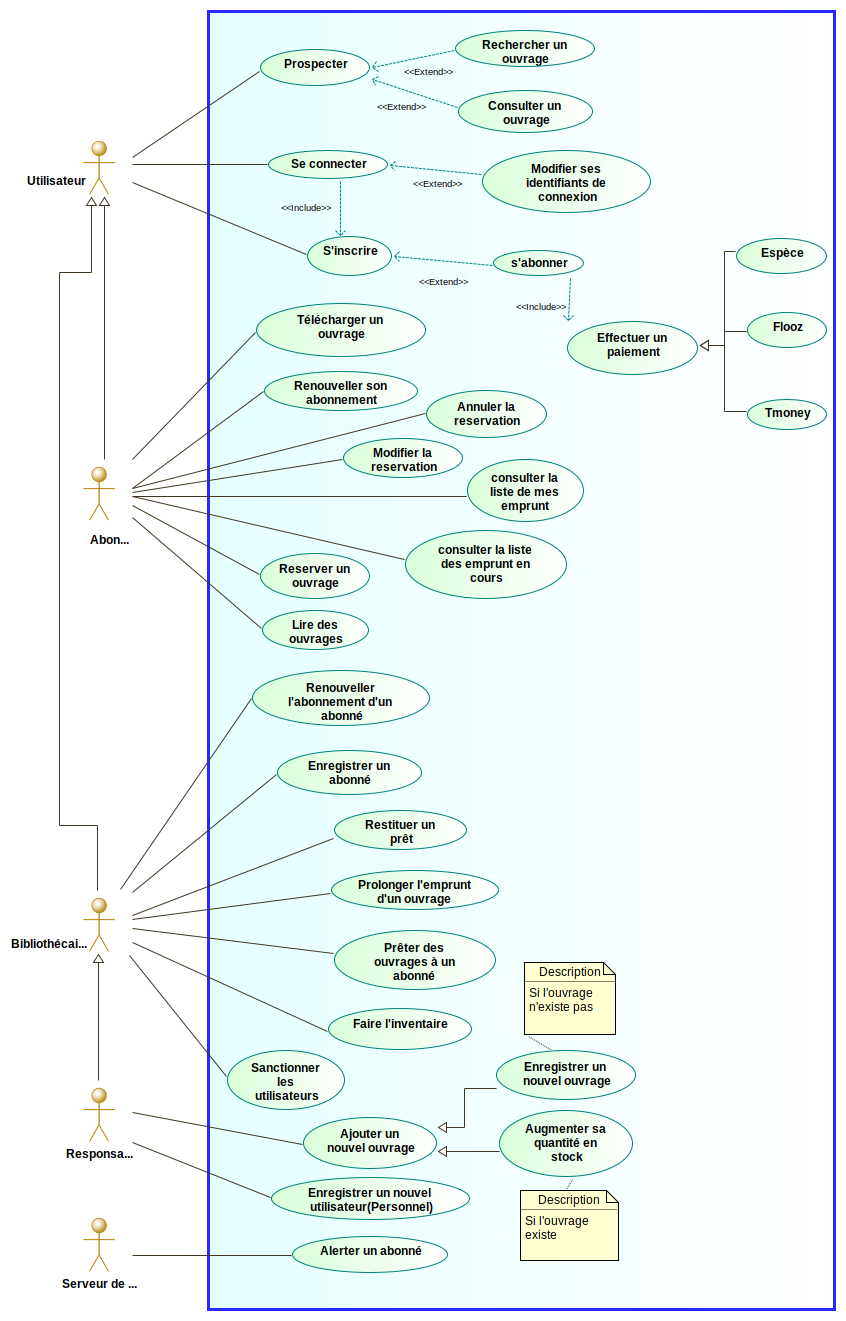
\includegraphics[scale=0.5]{images/UC.png}

\subsection{Diagramme de classe}
Le diagramme de classe quant à lui nous permet de représenter les données que nous 
allons manipuler afin de mieux les stocker dans une base de données et optimiser les multiples
façons de les traiter. Ici aussi nous nous sommes référé au cahier de charge et 
aux règles de gestion métier auxquelles nous avons apporté quelque ajout et changement.
Les voici :
\begin{itemize}
\item[•] Un ouvrage à un titre, un niveau, un type, une image, une langue, un résumer et
plusieurs mot clé.
\item[•] Un ouvrage peut être écrit par au moins un auteur et inversement un auteur peut
écrire plusieurs livres.
\item[•] Nous avons des ouvrages physique que nous pouvons approvisionner (qui sont
classé et rangé dans la bibliothèque) et des ouvrages électronique (qu'on peut 
télécharger) qui sont chacun pris individuellement des ouvrages.
\item[•] Parmi les ouvrages physique on compte les livres papier et documents
audiovisuelle et parmi les ouvrages électronique on peut compter les livres numérique
et les documents audiovisuelle électronique.
\item[•] Un utilisateur à un nom, un prénom, nom d'utilisateur, un mot de passe un 
contact, un profil, une adresse et un sexe.
\item[•] Parmi les utilisateurs on peut compter les abonnés qui ont en plus : une date
de naissance, un niveau d'étude, une carte d'identité ou scolaire, une profession et le
contact d'un proche et des personnels (employer de la médiathèque) qui ont un statu en 
plus. 
\item[•] Pour être abonné il faut payer un abonnement selon son niveau par divers moyen
a savoir : mobile money (T-money, Flooz) et le payement en liquide.
\item[•] Un abonné peut effectuer un emprunt ou une réservation et doit restituer
chaque emprunt.
\item[•] Un abonné a la possibilité de télécharger un ouvrage.
\end{itemize}
\newpage
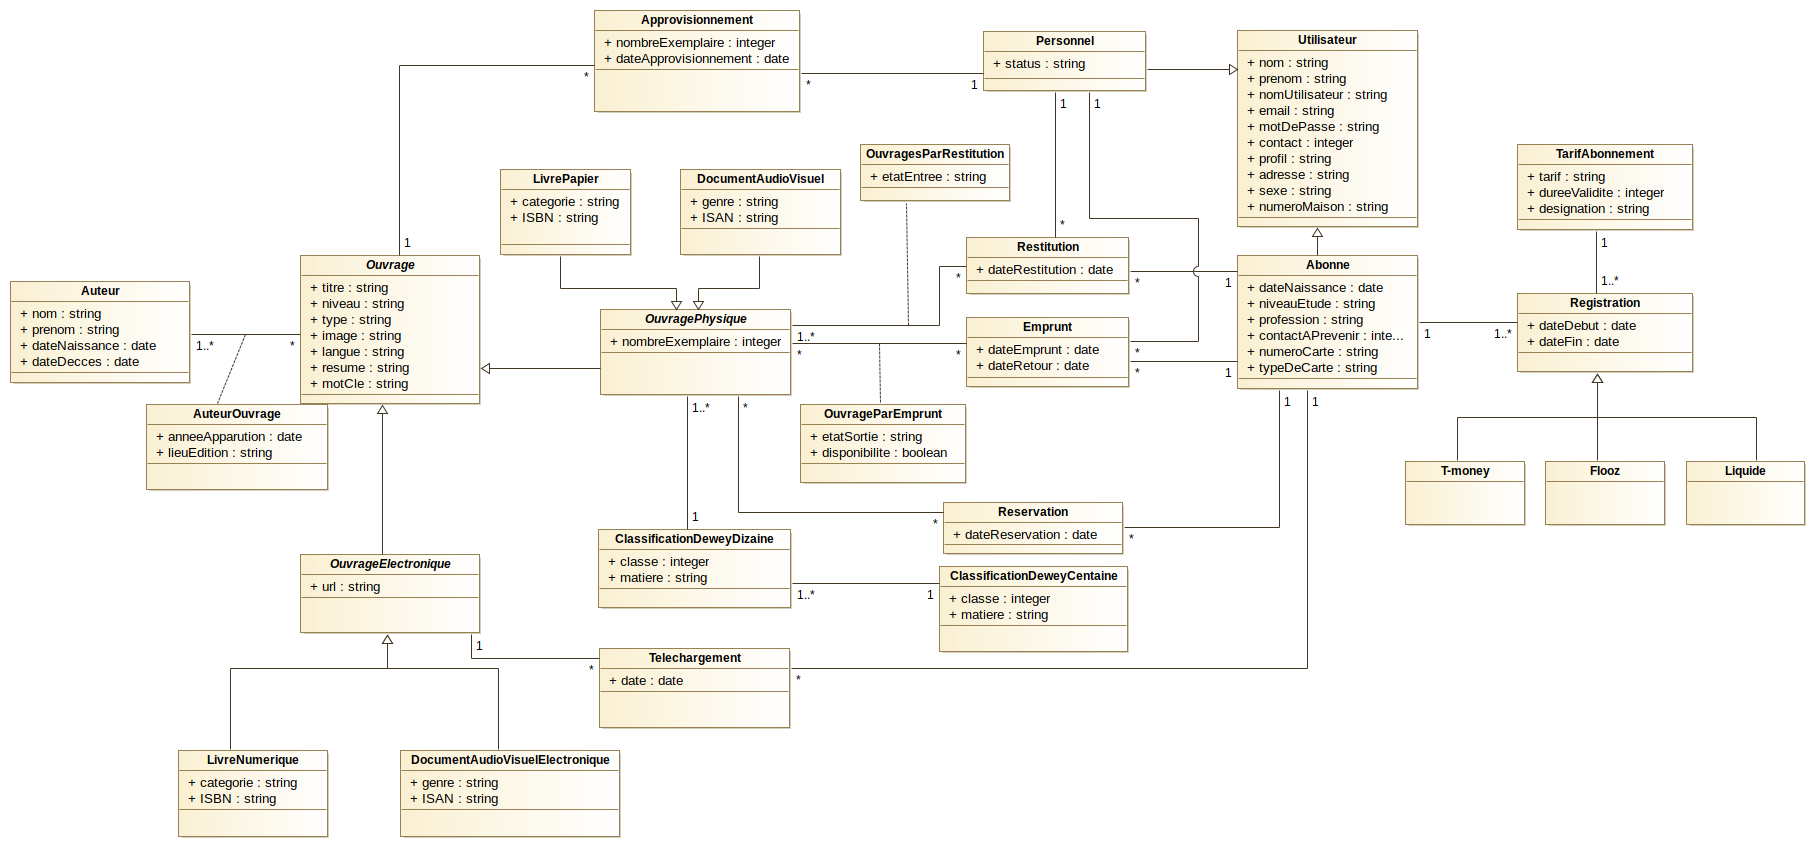
\includegraphics[scale=0.25]{images/CD.png}
\newpage
\subsection{Technologies et outils utilisé}
Au cours notre stage nous avons utiliser divers technologies et outils. Ici nous allons 
entrer plus en détails sur ces technologies et plus important encore nous allons 
expliquer la pertinence et le pourquoi de ces technologies.\\
\subsubsection{Technologie utilisé}
Parmi les technologies utilisé, nous pouvons citer : Laravel, PostgreSQL, Git...
\begin{itemize}
\item[•] UML : \\
C'est un Langage de Modélisation Unifier. C'est la toute première technologie que nous avons
utilisé il Nous à permis de mieux analyser le problème modéliser le problème au quelle
nous étions confronté. Nous l'avons choisit du fait de sont efficacité dans la modélisation
de données.
\item[•] PostgreSQL : \\
C'est un SGBD (Système de Gestion de base de données) nous avons choisit de l'utiliser
pour pouvoir stocker les données dans une base de donnée. Nous l'avons choisi car en
plus d'être une technologie apprise à l'institut, il est robuste, très efficace et plus
sûr.
\item[•] Laravel : \\
C'est un framework du langage de programmation php nous l'avons choisit car c'est une
technologie web et seul les technologie web sont capable de répondre efficacement aux besoins du
client (La médiathèque). De plus Laravel est la seul technologie web qu'on connais.
\item[•] JavaScript : \\
C'est un langage de programmation coté navigateur. Il nous a permit de rendre dynamique nos pages
web.
\item[•] Tailwind css : \\
C'est un framework css. C'est lui que nous avons utilisé pour styliser nos pages.
\end{itemize}
\subsubsection{Outils utilisé}
Parmi les outils utilisé, nous pouvons citer : Git , Planner, PHPStorm, VScode, Machine serveur.
\begin{itemize}
\item[•] Git : \\
C'est un gestionnaire de version. Il nous à permis de travailler efficacement en équipe en nous
permettant notamment de fusionner facilement notre travail et de travailler à distance. 
\item[•] Planner : \\
C'est un outils de gestion de projet. Il nous à permis comme vous pouvez aisément le deviner de 
gérer notre projet. Nous avons pu grâce à ce dernier faire une étude prévisionnelle du projet et faire
la répartition des tâches.
\item[•] PHPStorm \& Vscode : \\
Ce sont des \textbf{IDE (Environnement de Développement Intégré)} Ils nous ont permis de
travailler facilement, efficacement et rapidement sur notre projet mais nous vous conseillons 
d'utiliser PHPStorm car il est fait pour le développent en \textbf{PHP}.
\item[•] Machine Serveur : \\
C'est une machine sur laquelle nous avons hébergé notre site web.
\end{itemize}

\section{Réalisation}

\ Au cours de la période limité de notre stage sur les 26 classes énoncé dans notre diagramme de classe nous avons décidé de nous concentré et d'implémenter les classes que nous jugeons primordial et qui pourrons donner un excellent résultat. En effet sur les 26 classes proposé nous avons réussi à implémenter 19 classes dont la réalisation a été possible grâce au diagramme de cas d'utilisation établi. Cependant lors de l'établissement de notre diagramme de cas d'utilisation nous avons établi 5 acteurs et pour chaque acteur nous avons réussi à réaliser un certains nombre de ses cas d'utilisation. De ce fait concernant le premier acteur du système qui est l'utilisateur, sur toute ses cas d'utilisation nous avons réussi à implémenter 5 de ses cas d'utilisation; Pour ce qui est de notre deuxième acteur qui est l'abonne, nous avons réussi à implémenter 2 de ses cas d'utilisation; Concernant notre troisième acteur du système qui est la bibliothécaire, sur les cas d'utilisation dont elle dispose nous avons réussi à en effectuer 4; Pour ce qui est de notre quatrième acteur du système nous avons réussi à implémenter tous ses cas d'utilisation et pour le dernier acteur qui est le serveur de messagerie qui alertera un abonné au délai de son emprunt, nous avons pas encore implémenter ce cas d'utilisation. Ainsi grâce à l'implémentation de ces classes et cas d'utilisation, notre application procure quelques avantages tel qu'un utilisateur lambda peut venir consulter le site puis éventuellement s'inscrire et devenir un abonné afin de voir le contenu explicite d'un ouvrage. De plus le suivi de l'application est t'elle qu'un abonné peut aller sur l'application et emprunter un ouvrage ou même le restituer, effectuer une réservation d'un ouvrage, rechercher un ouvrage, télécharger un ouvrage, consulter un ouvrage et également lire un ouvrage. Grâce à l'application, le responsable de la bibliothèque qui s'occupe du bon déroulement de la bibliothèque et qui nomme la bibliothécaire peut ajouter un nouvel ouvrage, faire l'inventaire, enregistrer un nouvel employé. Aussi la bibliothécaire peut enregistrer un nouvel abonne, prolonger l'emprunt de cet abonné, prêter un ouvrage à un abonné, renouveler l'abonnement d'un abonné. En somme notre site web répond en grande partie au besoin exprimé par Urbis Foundation.
\section{Difficulté}
\subsection{Difficulté rencontré}
Au cours de notre stage de six semaine à la médiathèque, nous avons avons rencontré divers 
difficultés. certain d'ordre technique et d'autre d'ordre sociale.
\subsubsection{Difficulté technique}
Parmi les difficultés technique, nous pouvons citer le fait que Laravel n'était pas totalement
adapté pour résoudre notre problème du fais qu'il ne support pas des modèles basé sur l'héritage
de donnée. De ce fait il nous à été très difficile d'implémenter une partie de notre modèle.
Nous étions pas excellent en Laravel nous avons eu quasiment des problèmes à chaque
fois que nous devions implémenter quelque chose. En effet nous avons eu du mal à implémenter les 
relation du modèle surtout la relation \textbf{plusieurs à plusieurs}, modules comme la barre 
de débogage, le module d'import et export excel et le module de QrCode.\\
La deuxième difficulté était d'implémenter la recherche nous avons dépenser presque une semaine entière pour le faire.\\
Une autre difficulté était que notre application ne marchait que sur un navigateur
précis. Nous avons beaucoup de mal à résoudre ce problème. 

\subsubsection{Difficulté social} 
Parmi toute nos difficulté rencontrée tout au long de notre stage, la plus importante était sans doute d'ordre social. En effet nous avons fais deux 2/6 semaine plein à la médiathèque. Ceci à fais que nous nous sommes pas 
entièrement familiarisé avec le personnel de la médiathèque. De plus notre maître 
de stage était vraiment débordé ce qui à fais qu'il n'avait pas assez de temps à nous
consacré. Une autre difficulté d'ordre social était l'estimation du travail. Nous
avons estimer un travail à une semaine mais finalement nous y avons passé deux.Nous
étions aussi un peu stresser lors des présentations hebdomadaire que nous faisions avec le personnel et le cadre administratif de la médiathèque.\\

Toute ces difficulté ne nous ont pas submergé. Au contraire nous avons trouvé une 
solution à chacune d'elle notamment pour les difficultés d'ordre technique, la solution 
que nous avons trouvé à ces problèmes est le fait de suivi la documentation et pour ceux 
d'ordre sociale nous avons profité à fond des réunions hebdomadaires.

\subsection{Amélioration future}
A ce jour le projet n'est pas totalement terminé. Donc il est tout à fais logique de dire que
que nous allons déjà terminer notre application avant de commencer à l'améliorer.
Comme amélioration, nous avons prévus d'optimiser notre code pour que les pages se charge 
plus rapidement. Gérer l'abonnement via flooz et T-money.

\section{Conclusion}
Au demeurant notre stage à été parsemé d’embûche mais nous avons
toujours trouvé des solutions à nos problèmes. Nous avons adoré travailler pour
la médiathèque cela nous à permis d'amélioré nos compétences technique mais surtout professionnel,
compétence qui seront amélioré encore pendant la formation de prise en main de l'application qui se
tiendra à la médiathèque dans les jours avenir.

\end{document}



